\section{Численные алгоритмы решения прямых задач сложного теплообмена}
\label{sec:ch4/sec1}

\subsection{Метод Ньютона для стационарной модели}
\label{subsec:ch4/sec1/stationary}
Краевая задача сложного теплообмена
имеет вид (см. раздел~\ref{subsec:ch1/sec3/state})

\begin{equation}
    \label{eq:4_1:1}
        -a \Delta \theta+b \kappa_{a}| \theta|^{3} \theta =
        b \kappa_{a} \varphi,
\end{equation}
\begin{equation}
    \label{eq:4_1:2}
        -\alpha \Delta \varphi+\kappa_{a} \varphi =
        \kappa_{a}|\theta|^{3} \theta,
\end{equation}
\begin{equation}
    \label{eq:4_1:3}
        a \frac{\partial \theta}{\partial n}
        +\left.\beta\left(\theta-\theta_{b}\right)\right|_{\Gamma}=0,
        \quad \alpha \frac{\partial \varphi}{\partial n}
        +\left.\gamma\left(\varphi-\theta_{b}^{4}\right)\right|_{\Gamma}=0.
\end{equation}
Основную сложность при численном решении прямой задачи представляет нелинейность
по температурному полю, которое входит в систему
дифференциальных уравнений в четвёртой степени.

Метод простой итераций успешно применяется для решения задач в двумерной области.
Он был использован в работах~\cite{Kovtanyuk2015,astrakhantseva2014numerical}.
Однако, в трёхмерной области этот метод демонстрирует недостаточную скорость сходимости,
что приводит к долгим итерационным процессам и увеличению вычислительных затрат.

Вместо метода простой итераций для решения сложных задач оптимального управления
температурой может быть применен метод Ньютона.
Метод Ньютона является одним из наиболее эффективных методов оптимизации
и решения нелинейных уравнений.
Он использует локальную аппроксимацию функции в виде касательной плоскости
и обновляет решение на основе градиента и гессиана функции.
Этот метод обычно обеспечивает быструю сходимость и может быть
применен для решения сложных задач оптимального
управления температурой в трехмерных областях.


Метод Ньютона является усовершенствованным вариантом метода простой итерации,
в котором нелинейное слагаемое $|\theta|^3 \theta$ аппроксимируется
выражением $\widetilde{\theta}^4+4 \widetilde{\theta^3}(\theta-\widetilde{\theta})$,
где $\widetilde{\theta}$ - приближение для температуры на предыдущей итерации.
Эта аппроксимация обеспечивает более точное решение и быструю сходимость,
что делает метод Ньютона более эффективным для
решения задач с высокой степенью нелинейности.
В результате модифицированная система уравнений примет следующий вид:

\begin{equation}
    \tag{L1}
    \label{eq:L1}
    \begin{gathered}
        -a \Delta \theta+b \kappa_{a}\left(\left(4 \widetilde{\theta}^{3}
        \theta-3 \widetilde{\theta}^{4}\right)-\varphi\right)=0,\\
        \quad-\alpha \Delta \varphi
        +\kappa_{a}\left(\varphi
        -\left(4 \widetilde{\theta}^{3}
        \theta-3 \widetilde{\theta}^{4}\right)\right)=0;
    \end{gathered}
\end{equation}
\begin{equation}
     \tag{L2}
    \label{eq:L2}
        a \frac{\partial \theta}{\partial n}
        +\left.\beta\left(\theta-\theta_{b}\right)\right|_{\Gamma}=0,
        \quad \alpha \frac{\partial \varphi}{\partial n}
        +\left.\gamma\left(\varphi-\theta_{b}^{4}\right)\right|_{\Gamma}=0.
\end{equation}

Монотонная сходимость метода Ньютона является важным свойством,
которое позволяет обеспечить устойчивость итерационного процесса
и успешное решение эллиптических уравнений
с монотонным и выпуклым нелинейным слагаемым.
В литературе было проведено множество исследований, направленных
на изучение сходимости метода Ньютона для таких уравнений.

В частности, в работах~\cite{Mukhamadiev1971, Schryer1971} были представлены
результаты анализа монотонной сходимости метода Ньютона для эллиптического
уравнения с монотонным и выпуклым нелинейным слагаемым.
Результаты этих исследований показывают, что метод Ньютона обладает
хорошими свойствами сходимости и может быть применен для решения
сложных задач оптимального управления в моделях сложного теплообмена.

%\subsection{Квазистационарные и квазилинейные модели}
%\label{subsec:ch4/sec1/quasi}
%
%\textbf{Квазистационарная модель} радиационного и диффузионного теплообмена в ограниченной области
%$\Omega \subset \mathbb{R}^{3}$ с границей $\Gamma=\partial \Omega$
%в разделе~\ref{sec:ch2/sec3} представлена следующим образом
%
%\begin{align*}
%    & \frac{\partial \theta}{\partial t} - a \Delta \theta
%    + b \kappa_{a} \left(|\theta| \theta^{3}-\varphi\right) = 0,\\
%    & - \alpha \Delta \varphi
%    + \kappa_{a} \left(\varphi-|\theta| \theta^{3}\right) = 0, \\
%    \quad x \in \Omega, \quad 0 < t < T;
%    a \left(\partial_{n} \theta+\theta\right)=r, \\
%    \quad \alpha\left(\partial_{n} \varphi
%    + \varphi\right) = u \text { на } \Gamma;
%    \left.\theta\right|_{t=0} = \theta_{0}.
%\end{align*}
%
%
%
%Квазистационарная модель радиационного и диффузионного теплообмена в ограниченной области
%$\Omega \subset \mathbb{R}^{3}$ с границей $\Gamma=\partial \Omega$ в разделе~\ref{sec:ch3:sec3}
%\begin{gather*}
%    \sigma \partial \theta / \partial t-\operatorname{div}(k(\theta) \nabla \theta)
%    -\beta \varphi=u_{1} \chi, \\
%    \quad-\operatorname{div}(\alpha \nabla \varphi)+\beta \varphi= u_{2} \chi, \\
%    k(\theta) \partial_{n} \theta+\left.\gamma
%    \left(\theta-\theta_{b}\right)\right|_{\Gamma}=0,
%    \quad \alpha \partial_{n} \varphi +
%    \left.0.5 \varphi\right|_{\Gamma}=0,\left.\quad \theta\right|_{t=0}=\theta_{0}.
%        \quad x \in \Omega, \quad 0<t<T, \\
%\end{gather*}
%


\subsection{Примеры численного решения краевой задачи \eqref{eq:4_1:1}--\eqref{eq:4_1:3}}
\label{subsec:ch4/sec1/boundary}


Первым этапом решения задачи методом конечных элементов будет вывод слабой формулировки для
линеаризированной модели.
Для этого умножим уравнения~\eqref{eq:L1} на соответствующие тестовые функции
$v, \psi \in H^1(\Omega)$ и применим формулу Грина.
Учитывая краевые условия~\eqref{eq:L2}, получим:
\begin{equation*}
    \begin{aligned}
        & a( \nabla \theta, \nabla v ) + \int_\Gamma \beta \theta v d\Gamma
        + \left(b \kappa_a (| \theta | \theta^3 - \varphi ), v\right)
        = \int_\Gamma \beta \theta_b v d\Gamma,
        \\
        & \alpha (\nabla \varphi,\nabla \psi)
        + \int_{\Gamma_0 \cup \Gamma_2} \gamma \varphi v d\Gamma
        + \left( (\kappa_a (\varphi - |\theta|\theta^3), \psi\right)
        = \int_{\Gamma} \gamma \theta_b^4 \psi d\Gamma.
    \end{aligned}
\end{equation*}

\textbf{Пример 1} (двумерная область).
Положим $\Omega=\{(x,y),\, 0 \leq x,y \leq 1 \}$.

Метод конечных элементов требует разбиения области $\Omega$ на
конечное число непересекающихся подобластей, называющихся
\textit{конечными элементами}.
Отметим, что большинство современных солверов включают в себя
алгоритмы разбиения области на конечные элементы, а также подгрузку
уже разбитых областей.

Определим параметры системы следующим образом.
$a = 0.6$,
$\alpha = 0.333$,
$k_a = 1$,
$b = 0.025$,
$\beta = 1$,
$\gamma = 0.8 \cos\left(\frac{\pi}{2} y\right) + 0.5$,
$\theta_b = 0.1 + y / 2$.
Начальное приближение для функций $\theta$ и $\varphi$ выбрано нулевым.
Состояние, полученное за три итерации при данных параметрах представлено
на рисунке~\ref{fig:4_1:boundary}.
\begin{figure}[h!t]
    \begin{minipage}[b][][b]{0.49\linewidth}
        \centering
        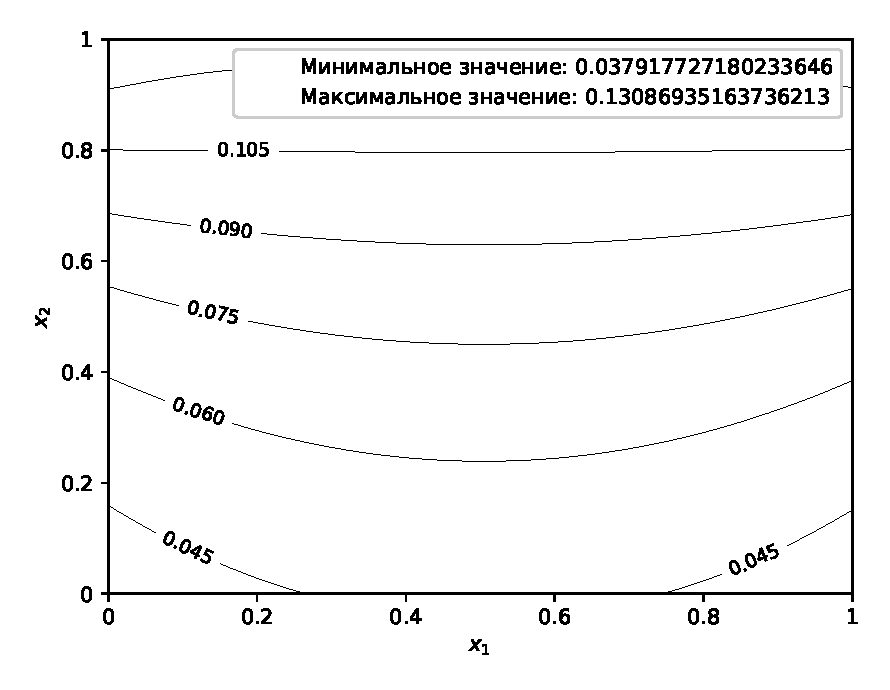
\includegraphics[width=1\linewidth]{boundary/theta_iso_auto} \\ а) $\theta$
    \end{minipage}
    \hfill
    \begin{minipage}[b][][b]{0.49\linewidth}
        \centering
        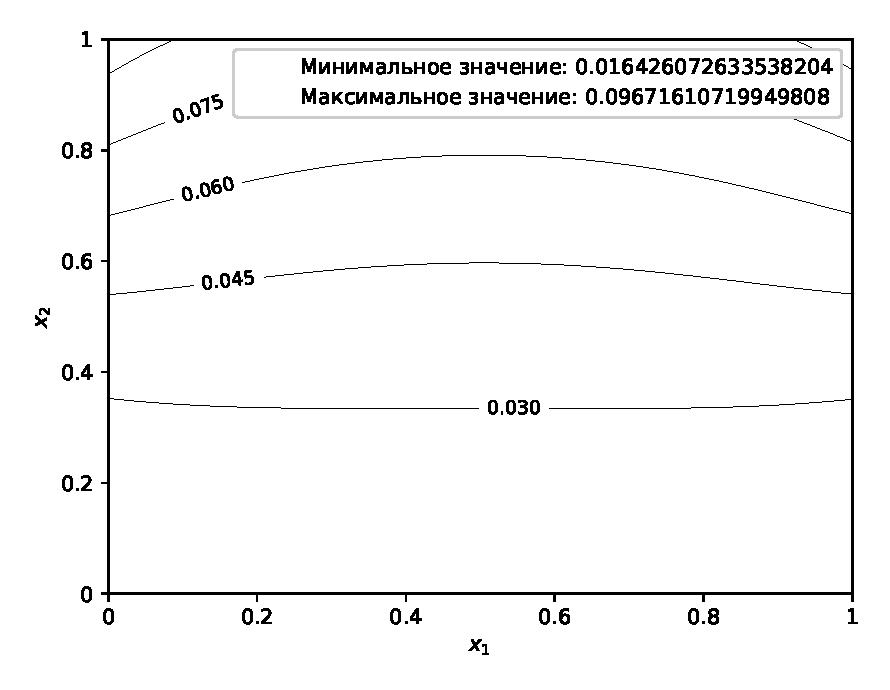
\includegraphics[width=1\linewidth]{boundary/phi_iso_auto} \\ б) $\varphi$
    \end{minipage}
    \caption{Решение граничной задачи в двумерной области}
    \label{fig:4_1:boundary}
\end{figure}


Код, используемый для получения решения представлен в приложении~\ref{lst:boundary}.
Инструментарий для получения изображений можно найти в репозитории~\cite{mesenev-github}.

\textbf{Пример 2} (трёхмерная область).
В таком случае область $\Omega=\{(x,y,z),\, 0 \leq x,y,z \leq 1 \}$.
Переопределим функции $\gamma, \theta_b$ следующим образом:
$\gamma = 0.8 \cos\left(\frac{\pi}{2} z\right) + 0.5$,
$\theta_b = 1- y / 2 + z /2$.

Начальное приближение также выбрано нулевым.
Для нахождения состояния потребовалось шесть итераций,
результат представлен на рисунке~\ref{fig:4_1:boundary_3d}.
\begin{figure}[h!t]
    \begin{minipage}[b][][b]{0.49\linewidth}
        \centering
        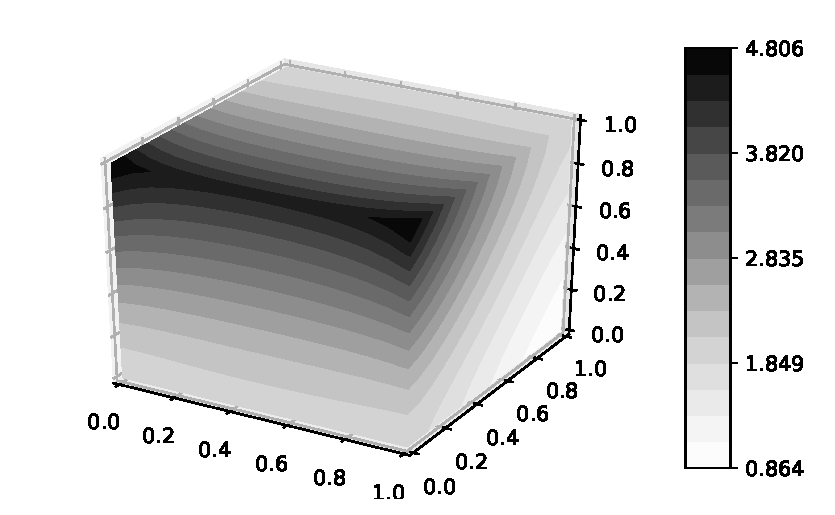
\includegraphics[width=1\linewidth]{boundary/theta_3d} \\ а) $\theta$
    \end{minipage}
    \hfill
    \begin{minipage}[b][][b]{0.49\linewidth}
        \centering
        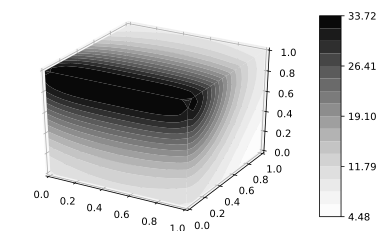
\includegraphics[width=1\linewidth]{boundary/phi_3d} \\ б) $\varphi$
    \end{minipage}
    \caption{Решение граничной задачи в трёхмерной области}
    \label{fig:4_1:boundary_3d}
\end{figure}

\begin{remark}
    Алгоритмы численного решения начально-краевых задач для квазилинейных моделей
    также основаны на продложенном выше методе Ньютона и будут изложены при описании
    алгоритмов решения обратных задач.
\end{remark}

